\documentclass[11pt,a4paper]{article}
\usepackage[T1]{fontenc}
\usepackage[utf8]{inputenc}
\usepackage{microtype}
\usepackage{amsmath,amssymb,amsfonts}
\usepackage{booktabs}
\usepackage{graphicx}
\usepackage{subcaption}
\usepackage{natbib}
\usepackage[colorlinks=true,linkcolor=blue,citecolor=blue,urlcolor=blue]{hyperref}
% cleveref errors if it is loaded before hyperref.
\usepackage[capitalize,noabbrev]{cleveref}

\title{Language as a latent port for LeWorldModel control on Push-T: a CPU probe of block angle}
\author{MMAGAI team\\Skoltech}
\date{}

\begin{document}
\maketitle

\begin{abstract}
This note asks whether block angle on Push-T is linearly readable in the frozen official LeWorldModel latent, including after a 180 degree turn.
The world model is the public \texttt{quentinll/lewm-pusht} checkpoint.
No language model sits inside the JEPA, and no goal image is generated from text.
Words are treated as a port onto objects that already live in the 192-dimensional embedding $z$.
On a CPU-only Xeon, a ridge probe from $z$ to $(\cos\theta,\sin\theta)$ has held-out mean absolute circular error 12.08 degrees on scripted 180 degree turns and 14.58 degrees on frames within 30 degrees of angle 0.
Under the pre-registered rule, 180 degrees is not a weak slice of this latent, so LeWorldModel is not finetuned.
A least-squares displacement $f(\mathrm{text})\in\mathbb{R}^{192}$ fit on the same turns does not beat predicting the mean residual scale of $\Delta z$.
\end{abstract}

\noindent\textbf{Keywords:}
LeWorldModel, JEPA, Push-T, linear probe, language interface.

\section{Introduction}
\label{sec:intro}
LeWorldModel (LeWM) is a joint-embedding predictive architecture trained from pixels with a next-embedding loss and a Gaussian regularizer \citep{maes2026lewm}.
The Push-T checkpoint used here was not trained with language, and this note does not put an LLM inside that JEPA.
The control story we want is closer to the latent-world-model programme in \citet{lecun2022path}: plan in a compact state, and attach language at that state rather than at pixels.
A practical port has to know which physical quantities are already linear in $z$.
Push-T's T-block angle $\theta$ is the quantity tested here, because a half-turn is a common failure mode for appearance-based embeddings that confuse $\theta$ with $\theta+\pi$.
The experiment is a frozen encoder, a scripted angle set, and a linear readout.
Cross-entropy method planning was not run.

\section{Related Work}
\label{sec:related}
\citet{lecun2022path} argues for autonomous intelligence built around a predictive world model in representation space, with separate modules for cost and action.
LeWM is one pixel-trained instance of that pattern: the published model encodes a $224\times 224$ RGB frame to a 192-dimensional vector and predicts future embeddings from actions \citep{maes2026lewm}.
GRIF aligns language with the change between observations rather than with a goal image, then trains a policy on that interface \citep{myers2023grif}.
The displacement head in \cref{sec:methods} is the same idea restricted to a frozen LeWM latent and to four template commands.
VL-JEPA predicts a continuous embedding of target text instead of autoregressive tokens \citep{chen2025vljepa}.
We do not train that model.
We only ask whether a text string can name a displacement that the frozen Push-T latent already contains.

\section{Methods}
\label{sec:methods}

\subsection{Hardware and frozen encoder}
The machine is an Intel Xeon E3-1270 v2 with 16 GB of RAM and no AVX2 or BMI2.
The GPU is an AMD RX 580 and was not used.
PyTorch is 2.14.0+cpu.
\texttt{torch.cuda.is\_available()} is false.
stable-worldmodel is 0.1.1 and transformers is 4.57.6.
Transformers 5 renames ViT parameters and cannot load this checkpoint.
The call is \texttt{load\_pretrained} on the repository id \texttt{quentinll/lewm-pusht}.
\texttt{STABLEWM\_HOME} points at the project data directory.
The module is set to eval mode on CPU.
Pixels follow \texttt{scripts/sanity\_encode.py}: uint8 HWC, scale to $[0,1]$, ImageNet mean and standard deviation, resize to 224, then a time axis so the tensor is $(B,1,3,224,224)$.
\texttt{encode(\{"pixels": pixels\})} returns \texttt{info["emb"]} with shape $(B,T,192)$.
One frame took 0.123 seconds, so the full set of 440 frames was encoded in batches of 8.
No frame was dropped for speed.
\texttt{eval.py} and CEM were not run.
The 13 GB Lance dataset and the 43 GB HDF5 archive were not downloaded.

\subsection{Push-T, headless}
The environment id is \texttt{swm/PushT-v1} with \texttt{render\_mode} set to \texttt{rgb\_array}.
The SDL video driver is dummy.
The matplotlib backend is Agg.
The pygame support prompt is hidden.
The MuJoCo GL backend variable is egl.
\texttt{render\_mode="human"} was not used.
A seed-0 reset is saved as \texttt{reset\_api.json}.
The unwrapped class is \texttt{PushT}.
Block pose in the info dict is $(x,y,\theta_{\mathrm{raw}})$ in pixels and radians.
\texttt{obs["state"]} is length 7: agent $xy$, block $xy$, block angle wrapped to $[0,2\pi)$, and agent velocity.
The goal overlay in that dump is fixed at $(256,256,\pi/4)$ because goal factors are not in the default randomization set.
Block angle is randomized on reset.
The variation-space initial value of block angle is 0, which is the origin used below for ``default pose''.
In-place turns call \texttt{PushT.\_set\_state} on the reset state with the block angle replaced by $\theta+\Delta\theta$ and agent velocity set to 0.
The setter writes the pymunk body and steps the space once.
Measured $xy$ after that step moved by 0.13 pixels on average and 3.78 pixels at most, against the paired random frame.

\subsection{Frame set and split}
Eighty episodes each contribute a random reset and three turns tagged \texttt{rot90}, \texttt{rot180}, and \texttt{rot\_m90} ($\Delta\theta\in\{+\pi/2,\pi,-\pi/2\}$).
One hundred and twenty further episodes are random resets only, so the official pose distribution is not only the bases of the turns.
The total is 440 frames.
Each row stores $z\in\mathbb{R}^{192}$, wrapped $\theta$ in radians and degrees, block $xy$, episode id, and the tag.
Files are \texttt{data/probes/pusht\_theta\_probe.npz} and \texttt{data/probes/pusht\_theta\_probe.csv}.
PNGs were not written.
Episodes are split 75/25 within each episode kind, seed 0, giving 150 train episodes (330 frames) and 50 test episodes (110 frames).
Frames from one episode never cross the split.

\subsection{Angle probe}
The probe predicts $(\cos\theta,\sin\theta)$, not the raw angle.
Ridge regression with $\alpha=1$ is the primary fit.
Ordinary least squares is reported beside it.
Predicted angle is $\mathrm{atan2}(\widehat{\sin\theta},\widehat{\cos\theta})$.
Circular error is the wrapped difference of that angle and the measured $\theta$, in degrees.
Mean absolute circular error (MAE) is the summary.
The decision rule, fixed before looking at a preferred slice, is: if held-out MAE on \texttt{rot180} frames is more than twice the MAE on frames with wrapped $|\theta|<30^{\circ}$, or if the \texttt{rot180} MAE exceeds 30 degrees, say that 180 degrees is weakly represented and a rental finetune of LeWM is justified.
Otherwise say that LeWM is not finetuned and only the language port is trained.
Plots use the matplotlib Agg backend and are saved as PDF.

\subsection{Language-port stub}
\texttt{scripts/language\_port.py} defines two interfaces that share one map $f$ from a command string to $\mathbb{R}^{192}$.
Displacement is
\begin{equation}
\hat{z}_{g} = z_{t} + f(\mathrm{text}).
\end{equation}
Energy is
\begin{equation}
E(z_{t}, z_{t+H}, \mathrm{text})
= \lVert (z_{t+H}-z_{t}) - f(\mathrm{text}) \rVert^{2}.
\end{equation}
The command list is ``rotate T 90'', ``rotate T 180'', ``rotate T -90'', and ``put T on the target''.
\texttt{CLIPTextModel} and \texttt{CLIPTokenizer} import on this CPU.
CLIP weights were not downloaded.
The fitted embedder is a four-way one-hot bag of commands.
$f(\mathrm{text})=W^{\top}e(\mathrm{text})$ is least squares of $\Delta z=z_{t+H}-z_{t}$ on that one-hot, using train episodes only.
Pairs are the three turns inside each rotation episode.
A pair is kept when the measured turn is within 20 degrees of the command and the block moves at most 5 pixels.
All 240 turn pairs passed.
``put T on the target'' has no same-$xy$ pair in this collection.
Its column of $W$ is the zero vector from the least-squares null space, and its residual is not measured.
No text-to-image model is trained.
The predictor is not conditioned on text.
\texttt{AutoCostModel} is not used.

\section{Results}
\label{sec:results}
\Cref{tab:mae} is the held-out circular MAE.
On the ridge probe, \texttt{rot180} MAE is 12.08 degrees ($n=20$) and the near-default slice $|\theta|<30^{\circ}$ has MAE 14.58 degrees ($n=19$).
The ratio is $12.08/14.58\approx 0.83$.
The \texttt{rot180} MAE is below 30 degrees.
The rule therefore says: do not finetune LeWM; only train the language port.
Ordinary least squares agrees on that sentence: its \texttt{rot180} MAE is 20.06 degrees and its near-default MAE is 26.09 degrees.
OLS test MAE on all 110 held-out frames is 18.88 degrees against a train MAE of 6.59 degrees, with train $(\cos,\sin)$ $R^{2}=0.958$.
Ridge test MAE is 13.75 degrees against a train MAE of 7.95 degrees, with train $R^{2}=0.935$.
Ridge is the probe cited by the decision because the test error is lower.
\Cref{fig:scatter} shows held-out predicted angle against wrapped true angle.
\Cref{fig:hist} shows the signed circular error inside eight bins of true $\theta$.
\Cref{fig:bins} and \cref{tab:bins} show MAE against absolute angle from 0.
No bin mean exceeds 30 degrees under ridge.
The noisiest ridge bin in that table is $[15,30)$ degrees, at 18.58 degrees with $n=6$.

\begin{table}[t]
\centering
\caption{Held-out mean absolute circular error in degrees.
Tags are the collection labels.
Near 0 means wrapped $|\theta|<30^{\circ}$.}
\label{tab:mae}
\begin{tabular}{lrrrr}
\toprule
Probe & random & rot90 & rot180 & rot$-90$ \\
\midrule
Ridge $\alpha=1$ & 12.36 & 16.17 & 12.08 & 16.50 \\
OLS & 19.91 & 16.90 & 20.06 & 17.09 \\
\bottomrule
\end{tabular}

\vspace{0.6em}
\begin{tabular}{lrr}
\toprule
Probe & all test & near 0 \\
\midrule
Ridge $\alpha=1$ & 13.75 ($n=110$) & 14.58 ($n=19$) \\
OLS & 18.88 ($n=110$) & 26.09 ($n=19$) \\
\bottomrule
\end{tabular}
\end{table}

\begin{table}[t]
\centering
\caption{Held-out ridge MAE by absolute wrapped angle from the default angle 0.}
\label{tab:bins}
\begin{tabular}{lrr}
\toprule
$|\theta|$ bin (deg) & $n$ & MAE (deg) \\
\midrule
$[0,15)$ & 13 & 12.74 \\
$[15,30)$ & 6 & 18.58 \\
$[30,45)$ & 11 & 12.51 \\
$[45,60)$ & 9 & 9.96 \\
$[60,90)$ & 16 & 13.42 \\
$[90,135)$ & 25 & 14.51 \\
$[135,180]$ & 30 & 14.36 \\
\bottomrule
\end{tabular}
\end{table}

\begin{figure}[t]
\centering
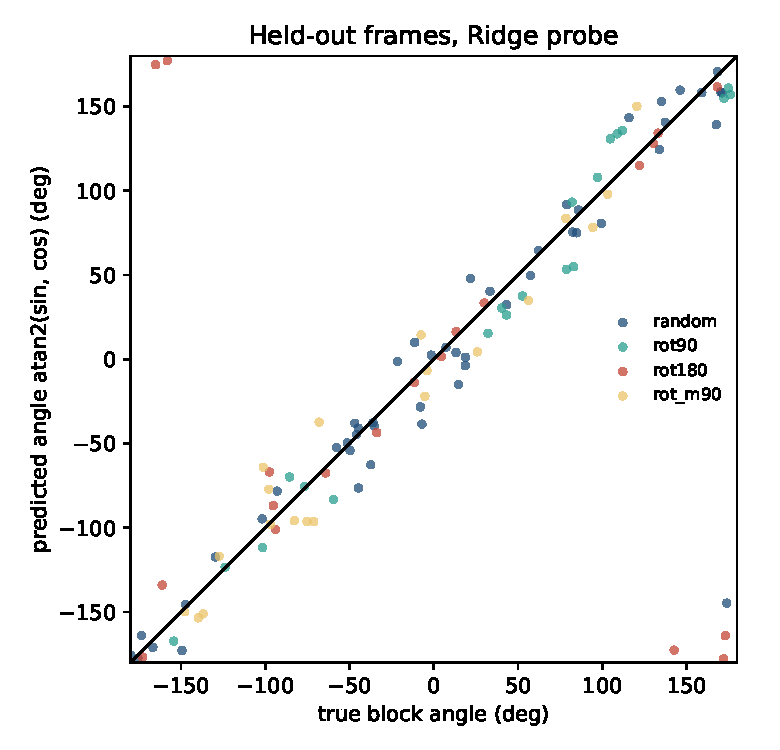
\includegraphics[width=0.72\linewidth]{figures/pred_vs_true_theta.pdf}
\caption{Held-out ridge predictions.
Both axes are wrapped to $[-180,180]$ degrees.
The line is equality.}
\label{fig:scatter}
\end{figure}

\begin{figure}[t]
\centering
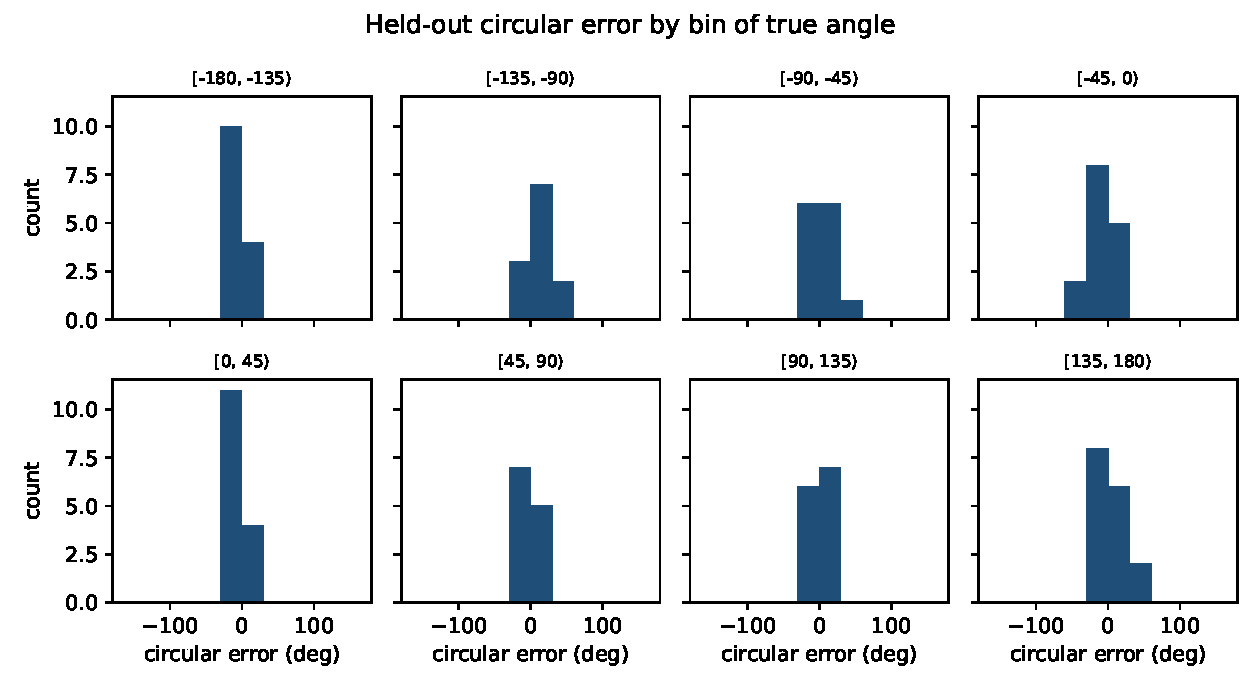
\includegraphics[width=\linewidth]{figures/error_hist_by_theta_bin.pdf}
\caption{Held-out signed circular error, one panel per bin of true wrapped angle.}
\label{fig:hist}
\end{figure}

\begin{figure}[t]
\centering
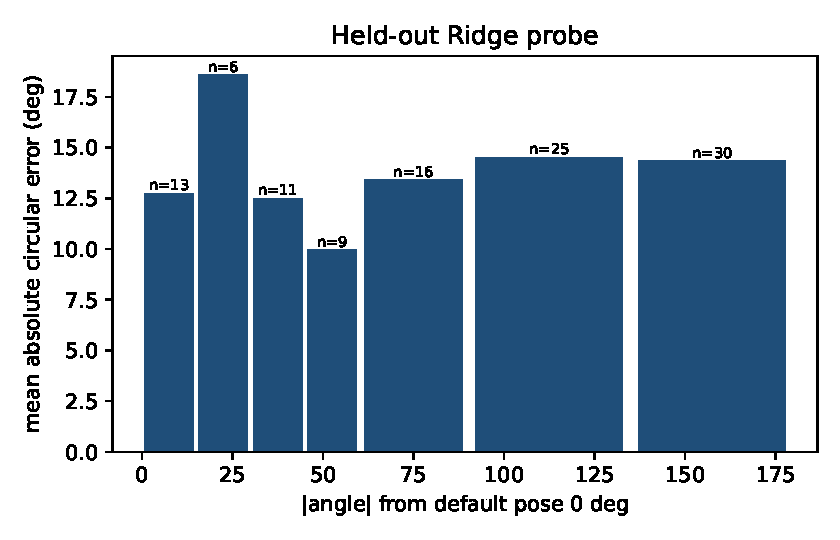
\includegraphics[width=0.78\linewidth]{figures/mae_vs_abs_dtheta.pdf}
\caption{Held-out ridge MAE against $|\theta|$ from angle 0.
Bar labels are bin counts.}
\label{fig:bins}
\end{figure}

The language port is a separate measurement.
Train RMSE of $\Delta z-f(\mathrm{text})$ is 1.089 per latent coordinate.
The RMS of $\Delta z$ itself is 1.099, so the ratio is 0.991.
Mean $\ell_{2}$ residual versus mean $\ell_{2}$ of $\Delta z$ is 13.41 versus 13.51 for ``rotate T 90'', 16.75 versus 16.89 for ``rotate T 180'', and 13.91 versus 13.99 for ``rotate T -90'', each on 60 train pairs.
Held-out RMSE is 1.197 on 60 pairs.
Mean held-out energy is 274.97.
``put T on the target'' is not measured, and $\|f\|$ for that string is 0.
A single vector per command does not account for the turn.
CEM success rate is not measured.

\section{Discussion}
\label{sec:discussion}
The angle readout does not get worse at a half turn.
Ridge MAE at \texttt{rot180} is slightly smaller than MAE near angle 0, and both sit near 12--15 degrees.
That is the region the decision rule treats as comparable, so the checkpoint's encoder is left frozen.
The same latent does not give a position-independent displacement for the template commands: $f(\mathrm{text})$ removes about one percent of the RMS of $\Delta z$.
Angle can be read by a linear map that sees $z$, while the difference $z(\theta+\Delta\theta)-z(\theta)$ still depends on where the block sits and on the base angle.
A language port that is only a lookup of $\Delta z$ is not a controller.
Training that port, if it is trained further, has to be a richer map than $f(\mathrm{text})$ alone.
This run does not justify spending a rental on a LeWM finetune for $\theta$.
The rental that is justified is a 24 GB NVIDIA host for CEM and for the Push-T training set, with \texttt{transformers} kept below version 5 until the checkpoint is re-exported.
The Lance and \texttt{kornia\_rs} wheels still SIGILL on this Xeon.
They were not required for the probe.
CLIP class imports succeeded and CLIP weights were not fetched.
Replacing the one-hot embedder with a frozen CLIP text tower is future work on a machine where that download is wanted.

\section{Conclusion}
\label{sec:conclusion}
On 440 headless Push-T frames, a frozen official LeWM encodes each frame to $z\in\mathbb{R}^{192}$ and a ridge probe reads $\theta$ with held-out MAE 13.75 degrees.
Scripted 180 degree frames are not the weak bin.
LeWM is not finetuned on the evidence of this probe.
The least-squares language displacement is fit and reported, and it does not explain $\Delta z$.
Full planning and the large datasets were left for a later GPU machine.

\appendix
\section{Reset API}
\label{app:api}
Seed 0 of \texttt{swm/PushT-v1} returns an \texttt{OrderEnforcing} wrapper around \texttt{PushT}.
Observation keys are \texttt{proprio} and \texttt{state}.
Info keys include the block pose, the goal pose, the goal state, agent position and velocity, a contact count, and a goal image.
\texttt{goal} is a $224\times 224\times 3$ uint8 image and was not stored in the probe table.
The goal pose in that dump is $(256, 256, 0.785)$.
Block pose in that dump is about $(383.77, 318.04, 4.97)$.
Turns use \texttt{\_set\_state}, which is present on the unwrapped env.

\bibliographystyle{plainnat}
\bibliography{refs}

\end{document}
